\documentclass[11pt,a4paper]{article}

\usepackage[spanish]{babel}
\usepackage[utf8]{inputenc}
\usepackage[T1]{fontenc}
\usepackage{lmodern}
\usepackage{geometry}
\geometry{margin=2.5cm}
\usepackage{graphicx}
\usepackage{booktabs}
\usepackage[]{float}
\usepackage{caption}
\usepackage{makecell}
\usepackage{hyperref}
\hypersetup{
	colorlinks=true,
	linkcolor=black,
	urlcolor=blue,
	citecolor=black
}

\title{Resumen del experimento TLS 1.3 PQC}
\author{José Luis Delgado Jiménez}
\date{\today}

\begin{document}
	\maketitle
	
	\section{Objetivo y alcance}
	
	Se han medido cuatro configuraciones de handshake TLS:
	
	\begin{itemize}
		\item C1: X25519 + certificado ECDSA clásico.
		\item C2: X25519MLKEM768 (híbrido) + certificado ECDSA clásico.
		\item C3: X25519 + certificado PQC (ML-DSA).
		\item C4: X25519MLKEM768 (híbrido) + certificado PQC.
	\end{itemize}
	
	Para cada escenario se han ejecutado \(N=100\,000\) handshakes sobre localhost, registrando latencias, volumen de datos y tiempo de CPU (task-clock) mediante perf stat.

	\section{Configuración experimental (resumen)}
	
	\begin{itemize}
		\item Stack criptográfico: OpenSSL 3 + oqsprovider.
		\item Servidor TLS: openssl s\_server con configuración específica por escenario.
		\item Cliente de prueba: tls\_bench\_client, que realiza \(N\) handshakes consecutivos y genera CSV con:
		\texttt{run\_id, elapsed\_ms, success, ssl\_error, bytes\_read, bytes\_written}.
		\item Métrica CPU: perf stat -x, -e task-clock, normalizada por handshake.
	\end{itemize}
	
	\section{Resultados}
	
	\subsection{Tamaño de certificados y claves}
	
	\begin{table}[H]
		\centering
		\caption{Tamaños de certificados y claves utilizadas.}
		\label{tab:cert_sizes_short}
		\begin{tabular}{lrr}
	\toprule
	file & size\_bytes & size\_kib \\
	\midrule
	ca\_classic.crt & 591 & 0.58 \\
	ca\_classic.key & 302 & 0.29 \\
	ca\_pqc.crt & 7521 & 7.34 \\
	ca\_pqc.key & 8196 & 8.00 \\
	server\_classic.crt & 570 & 0.56 \\
	server\_classic.key & 302 & 0.29 \\
	server\_pqc.crt & 7497 & 7.32 \\
	server\_pqc.key & 8196 & 8.00 \\
	\bottomrule
\end{tabular}

	\end{table}
	
	\begin{figure}[H]
		\centering
		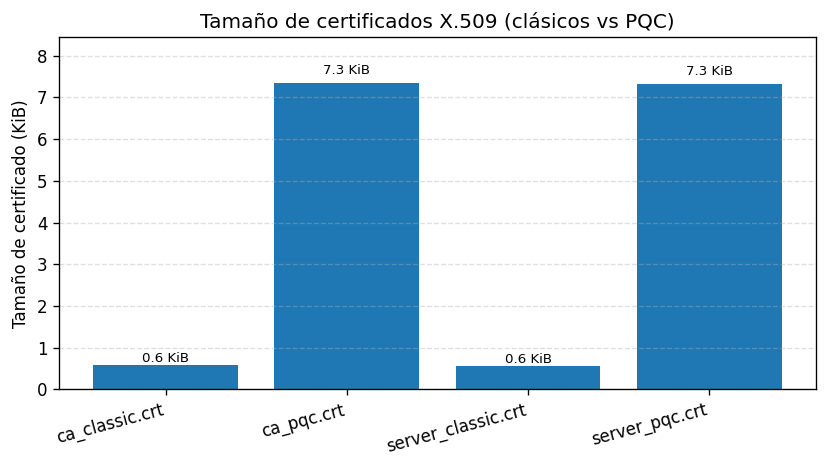
\includegraphics[width=\textwidth]{results/cert_sizes_bar.png}
		\caption{Tamaño de certificados X.509 clásicos vs post-cuánticos}
		\label{fig:cert_sizes_short}
	\end{figure}
	
	\subsection{Tamaño medio de handshake TLS 1.3}
	
	\begin{table}[H]
		\centering
		\caption{Tamaño medio del handshake TLS 1.3 por escenario}
		\label{tab:hs_size_short}
		\begin{tabular}{lrrrr}
	\toprule
	scenario & \makecell{bytes\_read} & \makecell{bytes\_written} & \makecell{handshake\_bytes} & std \\
	\midrule
	c1\_classic & 1318 & 402 & 1720 & 0.7 \\
	c2\_hybrid\_classiccert & 2406 & 1578 & 3984 & 0.7 \\
	c3\_classic\_pqcert & 14787 & 398 & 15185 & 0.0 \\
	c4\_hybrid\_pqcert & 15875 & 1574 & 17449 & 0.0 \\
	\bottomrule
\end{tabular}
	\end{table}
	
	\begin{figure}[H]
		\centering
		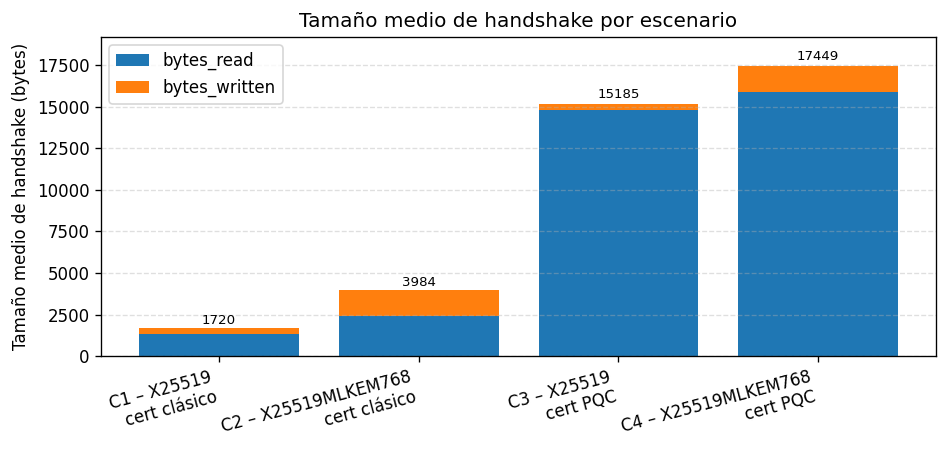
\includegraphics[width=\textwidth]{results/handshake_size_bar.png}
		\caption{Tamaño medio de handshake TLS 1.3 (bytes leídos vs escritos)}
		\label{fig:hs_size_bar_short}
	\end{figure}
	
	\subsection{Latencias de handshake}
	
	\begin{table}[H]
		\centering
		\caption{Estadísticos de latencia de handshake TLS 1.3 en ms.}
		\label{tab:latency_short}
		\begin{tabular}{lrrrrrr}
	\toprule
	scenario & N & mean\_ms & std\_ms & min\_ms & p50\_ms & p75\_ms \\
	\midrule
	c1\_classic & 100000 & 1.492 & 0.630 & 0.684 & 1.392 & 1.670 \\
	c2\_hybrid\_classiccert & 100000 & 1.890 & 0.694 & 0.839 & 1.775 & 2.112 \\
	c3\_classic\_pqcert & 100000 & 1.311 & 0.422 & 0.682 & 1.221 & 1.507 \\
	c4\_hybrid\_pqcert & 100000 & 1.490 & 0.490 & 0.858 & 1.363 & 1.680 \\
	\bottomrule
\end{tabular}

\vspace{1em}

\begin{tabular}{lrrrrrr}
	\toprule
	p90\_ms & p95\_ms & p99\_ms & max\_ms & overhead\_mean\_C1\_\% & overhead\_p99\_C1\_\% \\
	\midrule
	2.030 & 2.315 & 3.063 & 45.554 & 0.000 & 0.000 \\
	2.562 & 2.879 & 3.766 & 37.768 & 26.652 & 22.951 \\
	1.779 & 1.969 & 2.685 & 27.193 & -12.114 & -12.341 \\
	2.013 & 2.270 & 3.058 & 31.729 & -0.135 & -0.164 \\
	\bottomrule
\end{tabular}
	\end{table}
	
	\vspace*{4em}
	
	\begin{figure}[H]
		\centering
		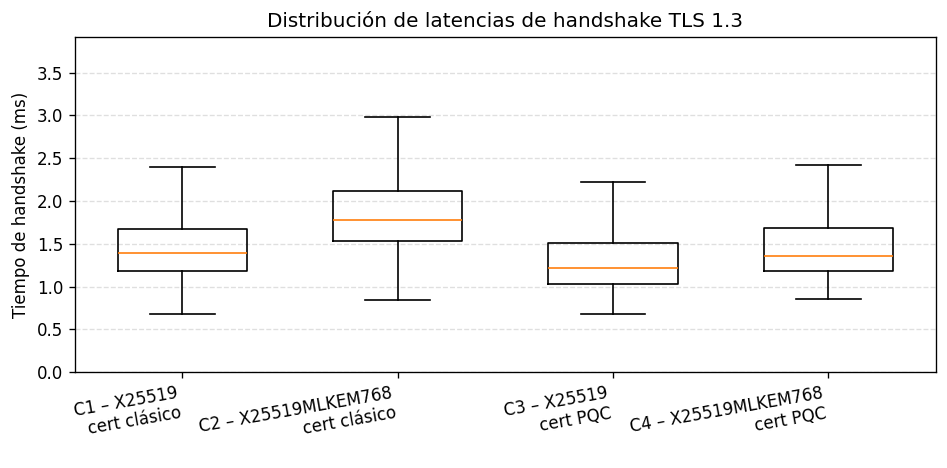
\includegraphics[width=\textwidth]{results/latency_boxplot.png}
		\caption{Distribución de latencias de handshake TLS 1.3 por escenario}
		\label{fig:latency_boxplot_short}
	\end{figure}
	
	\begin{figure}[H]
		\centering
		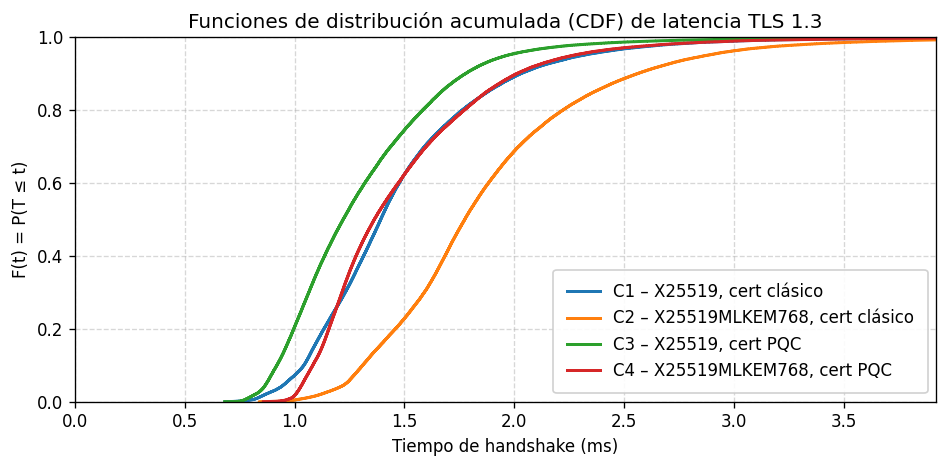
\includegraphics[width=\textwidth]{results/latency_cdf.png}
		\caption{Funciones de distribución acumulada (CDF) de latencia}
		\label{fig:latency_cdf_short}
	\end{figure}
	
	\vspace*{5em}
	
	\subsection{Tiempo de CPU por handshake}
	
	\begin{table}[H]
		\centering
		\caption{Tiempo de CPU (task-clock) y tamaño medio de handshake}
		\label{tab:cpu_short}
		\begin{tabular}{lrrr}
	\toprule
	scenario & bytes\_read\_mean & bytes\_written\_mean & task\_clock\_total \\
	\midrule
	c1\_classic & 1317.994 & 402 & 1.056e11 \\
	c2\_hybrid\_classiccert & 2405.995 & 1578 & 1.306e11 \\
	c3\_classic\_pqcert & 14787 & 398 & 9.456e10 \\
	c4\_hybrid\_pqcert & 15875 & 1574 & 1.035e11 \\
	\bottomrule
\end{tabular}

\vspace{1em}

\begin{tabular}{rr}
	\toprule
	task\_clock\_per\_hs & overhead\_cpu\_per\_hs\_vs\_C1\_\% \\
	\midrule
	1055613.185 & 0.000 \\
	1305993.180 & 23.719 \\
	945553.206 & -10.426 \\
	1035110.372 & -1.942 \\
	\bottomrule
\end{tabular}
	\end{table}
	
	\begin{figure}[H]
		\centering
		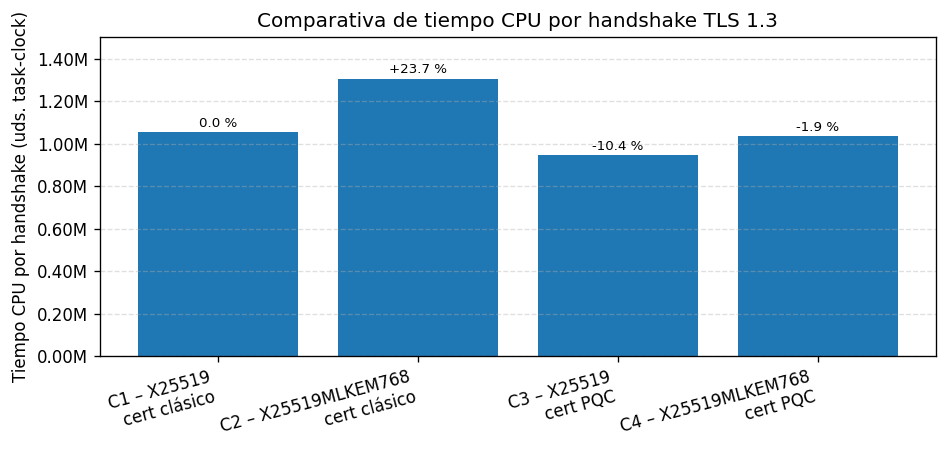
\includegraphics[width=\textwidth]{results/cpu_time_per_handshake_bar.png}
		\caption{Tiempo de CPU por handshake TLS 1.3 (baseline C1)}
		\label{fig:cpu_bar_short}
	\end{figure}
	
		\vspace*{3em}
	
	\section{Resumen}
	
	\begin{itemize}
		\item Los certificados y claves PQC ocupan aproximadamente un orden de magnitud más que los clásicos (del orden de 0{,}6~KiB frente a 7--8~KiB por certificado/clave).
		\item El tamaño medio del handshake TLS 1.3 pasa de unos 1{,}7~KiB en el escenario clásico (C1) a aproximadamente 4~KiB en el escenario híbrido con certificado clásico (C2) y a unos 15--17~KiB en los escenarios con certificados PQC (C3, C4).
		\item Las latencias de handshake se sitúan, según tabla \ref{tab:latency_short}, en torno a 1{,}3--1{,}9~ms de media, con percentiles 99 en el entorno de 3~ms.
		\item El tiempo de CPU por handshake se incrementa aproximadamente un 24\% en el escenario híbrido con certificado clásico (C2) y se mantiene similar o algo por debajo del clásico en los escenarios con certificado PQC (C3, C4), según tabla \ref{tab:cpu_short} y figura \ref{fig:cpu_bar_short}.
	\end{itemize}
	
\end{document}